% Options for packages loaded elsewhere
\PassOptionsToPackage{unicode}{hyperref}
\PassOptionsToPackage{hyphens}{url}
%
\documentclass[
  ignorenonframetext,
]{beamer}
\usepackage{pgfpages}
\setbeamertemplate{caption}[numbered]
\setbeamertemplate{caption label separator}{: }
\setbeamercolor{caption name}{fg=normal text.fg}
\beamertemplatenavigationsymbolsempty
% Prevent slide breaks in the middle of a paragraph
\widowpenalties 1 10000
\raggedbottom
\setbeamertemplate{part page}{
  \centering
  \begin{beamercolorbox}[sep=16pt,center]{part title}
    \usebeamerfont{part title}\insertpart\par
  \end{beamercolorbox}
}
\setbeamertemplate{section page}{
  \centering
  \begin{beamercolorbox}[sep=12pt,center]{part title}
    \usebeamerfont{section title}\insertsection\par
  \end{beamercolorbox}
}
\setbeamertemplate{subsection page}{
  \centering
  \begin{beamercolorbox}[sep=8pt,center]{part title}
    \usebeamerfont{subsection title}\insertsubsection\par
  \end{beamercolorbox}
}
\AtBeginPart{
  \frame{\partpage}
}
\AtBeginSection{
  \ifbibliography
  \else
    \frame{\sectionpage}
  \fi
}
\AtBeginSubsection{
  \frame{\subsectionpage}
}

\usepackage{amsmath,amssymb}
\usepackage{iftex}
\ifPDFTeX
  \usepackage[T1]{fontenc}
  \usepackage[utf8]{inputenc}
  \usepackage{textcomp} % provide euro and other symbols
\else % if luatex or xetex
  \usepackage{unicode-math}
  \defaultfontfeatures{Scale=MatchLowercase}
  \defaultfontfeatures[\rmfamily]{Ligatures=TeX,Scale=1}
\fi
\usepackage{lmodern}
\ifPDFTeX\else
    % xetex/luatex font selection
\fi
% Use upquote if available, for straight quotes in verbatim environments
\IfFileExists{upquote.sty}{\usepackage{upquote}}{}
\IfFileExists{microtype.sty}{% use microtype if available
  \usepackage[]{microtype}
  \UseMicrotypeSet[protrusion]{basicmath} % disable protrusion for tt fonts
}{}
\makeatletter
\@ifundefined{KOMAClassName}{% if non-KOMA class
  \IfFileExists{parskip.sty}{%
    \usepackage{parskip}
  }{% else
    \setlength{\parindent}{0pt}
    \setlength{\parskip}{6pt plus 2pt minus 1pt}}
}{% if KOMA class
  \KOMAoptions{parskip=half}}
\makeatother
\usepackage{xcolor}
\newif\ifbibliography
\setlength{\emergencystretch}{3em} % prevent overfull lines
\setcounter{secnumdepth}{-\maxdimen} % remove section numbering

\usepackage{color}
\usepackage{fancyvrb}
\newcommand{\VerbBar}{|}
\newcommand{\VERB}{\Verb[commandchars=\\\{\}]}
\DefineVerbatimEnvironment{Highlighting}{Verbatim}{commandchars=\\\{\}}
% Add ',fontsize=\small' for more characters per line
\usepackage{framed}
\definecolor{shadecolor}{RGB}{241,243,245}
\newenvironment{Shaded}{\begin{snugshade}}{\end{snugshade}}
\newcommand{\AlertTok}[1]{\textcolor[rgb]{0.68,0.00,0.00}{#1}}
\newcommand{\AnnotationTok}[1]{\textcolor[rgb]{0.37,0.37,0.37}{#1}}
\newcommand{\AttributeTok}[1]{\textcolor[rgb]{0.40,0.45,0.13}{#1}}
\newcommand{\BaseNTok}[1]{\textcolor[rgb]{0.68,0.00,0.00}{#1}}
\newcommand{\BuiltInTok}[1]{\textcolor[rgb]{0.00,0.23,0.31}{#1}}
\newcommand{\CharTok}[1]{\textcolor[rgb]{0.13,0.47,0.30}{#1}}
\newcommand{\CommentTok}[1]{\textcolor[rgb]{0.37,0.37,0.37}{#1}}
\newcommand{\CommentVarTok}[1]{\textcolor[rgb]{0.37,0.37,0.37}{\textit{#1}}}
\newcommand{\ConstantTok}[1]{\textcolor[rgb]{0.56,0.35,0.01}{#1}}
\newcommand{\ControlFlowTok}[1]{\textcolor[rgb]{0.00,0.23,0.31}{\textbf{#1}}}
\newcommand{\DataTypeTok}[1]{\textcolor[rgb]{0.68,0.00,0.00}{#1}}
\newcommand{\DecValTok}[1]{\textcolor[rgb]{0.68,0.00,0.00}{#1}}
\newcommand{\DocumentationTok}[1]{\textcolor[rgb]{0.37,0.37,0.37}{\textit{#1}}}
\newcommand{\ErrorTok}[1]{\textcolor[rgb]{0.68,0.00,0.00}{#1}}
\newcommand{\ExtensionTok}[1]{\textcolor[rgb]{0.00,0.23,0.31}{#1}}
\newcommand{\FloatTok}[1]{\textcolor[rgb]{0.68,0.00,0.00}{#1}}
\newcommand{\FunctionTok}[1]{\textcolor[rgb]{0.28,0.35,0.67}{#1}}
\newcommand{\ImportTok}[1]{\textcolor[rgb]{0.00,0.46,0.62}{#1}}
\newcommand{\InformationTok}[1]{\textcolor[rgb]{0.37,0.37,0.37}{#1}}
\newcommand{\KeywordTok}[1]{\textcolor[rgb]{0.00,0.23,0.31}{\textbf{#1}}}
\newcommand{\NormalTok}[1]{\textcolor[rgb]{0.00,0.23,0.31}{#1}}
\newcommand{\OperatorTok}[1]{\textcolor[rgb]{0.37,0.37,0.37}{#1}}
\newcommand{\OtherTok}[1]{\textcolor[rgb]{0.00,0.23,0.31}{#1}}
\newcommand{\PreprocessorTok}[1]{\textcolor[rgb]{0.68,0.00,0.00}{#1}}
\newcommand{\RegionMarkerTok}[1]{\textcolor[rgb]{0.00,0.23,0.31}{#1}}
\newcommand{\SpecialCharTok}[1]{\textcolor[rgb]{0.37,0.37,0.37}{#1}}
\newcommand{\SpecialStringTok}[1]{\textcolor[rgb]{0.13,0.47,0.30}{#1}}
\newcommand{\StringTok}[1]{\textcolor[rgb]{0.13,0.47,0.30}{#1}}
\newcommand{\VariableTok}[1]{\textcolor[rgb]{0.07,0.07,0.07}{#1}}
\newcommand{\VerbatimStringTok}[1]{\textcolor[rgb]{0.13,0.47,0.30}{#1}}
\newcommand{\WarningTok}[1]{\textcolor[rgb]{0.37,0.37,0.37}{\textit{#1}}}

\providecommand{\tightlist}{%
  \setlength{\itemsep}{0pt}\setlength{\parskip}{0pt}}\usepackage{longtable,booktabs,array}
\usepackage{calc} % for calculating minipage widths
\usepackage{caption}
% Make caption package work with longtable
\makeatletter
\def\fnum@table{\tablename~\thetable}
\makeatother
\usepackage{graphicx}
\makeatletter
\def\maxwidth{\ifdim\Gin@nat@width>\linewidth\linewidth\else\Gin@nat@width\fi}
\def\maxheight{\ifdim\Gin@nat@height>\textheight\textheight\else\Gin@nat@height\fi}
\makeatother
% Scale images if necessary, so that they will not overflow the page
% margins by default, and it is still possible to overwrite the defaults
% using explicit options in \includegraphics[width, height, ...]{}
\setkeys{Gin}{width=\maxwidth,height=\maxheight,keepaspectratio}
% Set default figure placement to htbp
\makeatletter
\def\fps@figure{htbp}
\makeatother

\makeatletter
\@ifpackageloaded{caption}{}{\usepackage{caption}}
\AtBeginDocument{%
\ifdefined\contentsname
  \renewcommand*\contentsname{Table of contents}
\else
  \newcommand\contentsname{Table of contents}
\fi
\ifdefined\listfigurename
  \renewcommand*\listfigurename{List of Figures}
\else
  \newcommand\listfigurename{List of Figures}
\fi
\ifdefined\listtablename
  \renewcommand*\listtablename{List of Tables}
\else
  \newcommand\listtablename{List of Tables}
\fi
\ifdefined\figurename
  \renewcommand*\figurename{Figure}
\else
  \newcommand\figurename{Figure}
\fi
\ifdefined\tablename
  \renewcommand*\tablename{Table}
\else
  \newcommand\tablename{Table}
\fi
}
\@ifpackageloaded{float}{}{\usepackage{float}}
\floatstyle{ruled}
\@ifundefined{c@chapter}{\newfloat{codelisting}{h}{lop}}{\newfloat{codelisting}{h}{lop}[chapter]}
\floatname{codelisting}{Listing}
\newcommand*\listoflistings{\listof{codelisting}{List of Listings}}
\makeatother
\makeatletter
\makeatother
\makeatletter
\@ifpackageloaded{caption}{}{\usepackage{caption}}
\@ifpackageloaded{subcaption}{}{\usepackage{subcaption}}
\makeatother

\ifLuaTeX
  \usepackage{selnolig}  % disable illegal ligatures
\fi
\usepackage{bookmark}

\IfFileExists{xurl.sty}{\usepackage{xurl}}{} % add URL line breaks if available
\urlstyle{same} % disable monospaced font for URLs
\hypersetup{
  pdftitle={Sensitivity Analysis of Spatial Scale and Particle Density on Overland Flow Pattern Accuracy and Computational Demand},
  pdfauthor={Corey White; Caitlin Haedrich; Helena Mitasova},
  hidelinks,
  pdfcreator={LaTeX via pandoc}}


\title{Sensitivity Analysis of Spatial Scale and Particle Density on
Overland Flow Pattern Accuracy and Computational Demand}
\subtitle{AGU 2024, Washington D.C}
\author{Corey White \and Caitlin Haedrich \and Helena Mitasova}
\date{2024-12-12}

\begin{document}
\frame{\titlepage}


\begin{frame}{What is SIMWE?}
\phantomsection\label{what-is-simwe}
\textbf{SIMWE} (SIMulation of Water Erosion Model) is a spatially
distributed processes-based overland flow model that simulates water
flow.

\begin{block}{How does SIMWE work?}
\phantomsection\label{how-does-simwe-work}
\begin{columns}[T]
\begin{column}{0.6\textwidth}
SIMWE uses \textbf{Green's function} to solve the \textbf{St.~Venant
system of equations} via a \textbf{Monte Carlo path sampling method}.
\end{column}

\begin{column}{0.4\textwidth}
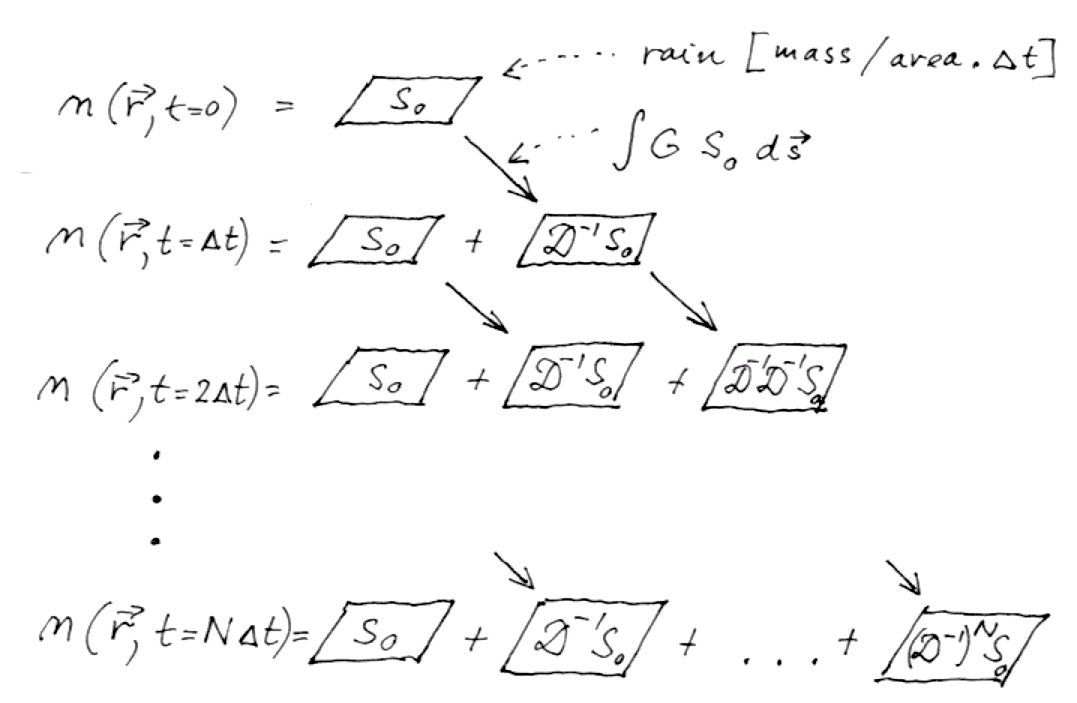
\includegraphics{images/evolfig.jpg}
\end{column}
\end{columns}
\end{block}
\end{frame}

\begin{frame}{Why this method?}
\phantomsection\label{why-this-method}
Water flows according to the shallow water bivariate \textbf{continuity
equation} (mass conservation), incorporating \textbf{drift} and
\textbf{diffusion}, which allows the \textbf{elevation model} to remain
\textbf{unmodified} (e.g., no sink and fill processing).
\end{frame}

\begin{frame}
\begin{block}{Path Sampling Method}
\phantomsection\label{path-sampling-method}
Solution of SWF equation incorporates spatially variable flow velocity

\begin{itemize}
\tightlist
\item
  \textbf{Variable rainfall excess} (impact of soils and land cover on
  infiltration),
\item
  \textbf{Topography} (slope steepness)
\item
  \textbf{Land cover} (Mannings roughness coefficient)
\end{itemize}
\end{block}

\begin{block}{Computational Demands of Overland Flow Modeling?}
\phantomsection\label{computational-demands-of-overland-flow-modeling}
The accuracy of overland flow simulations using path sampling methods
depends heavily on particle density. However, varying particle density
and spatial scale can be computationally demanding.

\begin{quote}
Error is proportional to \(1/\sqrt{N}\) where \(N\) is number of
particles.
\end{quote}
\end{block}

\begin{block}{Why is this a problem?}
\phantomsection\label{why-is-this-a-problem}
\begin{columns}[T]
\begin{column}{0.5\textwidth}
\begin{itemize}
\tightlist
\item
  Restrictive for research and policy development
\end{itemize}

\begin{itemize}
\tightlist
\item
  Emergency management applications require rapid response times
\end{itemize}

\begin{itemize}
\tightlist
\item
  Accuracy depends on particle density
\end{itemize}

\begin{itemize}
\tightlist
\item
  Spatial scale influences particle density required for accurate
  results
\end{itemize}
\end{column}

\begin{column}{0.5\textwidth}
\includegraphics{../notebooks/output/clay-center_depth_1_1_s_prob.webp}
\end{column}
\end{columns}
\end{block}
\end{frame}

\begin{frame}[fragile]{How did we approach this problem?}
\phantomsection\label{how-did-we-approach-this-problem}
\begin{block}{Software}
\phantomsection\label{software}
\begin{columns}[T]
\begin{column}{0.4\textwidth}
\end{column}

\begin{column}{0.6\textwidth}
\begin{itemize}
\item
  GRASS GIS v8.5
\item
  Geospatial Processing Engine
\item
  C and Python APIs
\item
  Open Source GPL v3
\item
  Parallelized (OpenMP)
\item
  SIMWE implemented as GRASS module \textbf{r.sim.water}
\end{itemize}
\end{column}
\end{columns}
\end{block}

\begin{block}{Computational Resources}
\phantomsection\label{computational-resources}
\begin{longtable}[]{@{}ll@{}}
\toprule\noalign{}
\textbf{Component} & \textbf{Specification} \\
\midrule\noalign{}
\endhead
\textbf{Laptop} & System76 Serval WS \\
\textbf{OS Name} & Pop!\_OS 22.04 LTS \\
\textbf{OS Type} & 64-bit \\
\textbf{Memory} & 64.0 GiB \\
\textbf{Processor} & 13th Gen Intel® Core™ i9-13900HX × 32 \\
\textbf{Graphics} & NVIDIA Corporation / Mesa Intel® Graphics (RPL-S) \\
\textbf{Disk Capacity} & 8.0 TB \\
\bottomrule\noalign{}
\end{longtable}
\end{block}

\begin{block}{Model Parameterization}
\phantomsection\label{model-parameterization}
\begin{columns}[T]
\begin{column}{0.5\textwidth}
\begin{block}{Spatially Uniform Parameters}
\phantomsection\label{spatially-uniform-parameters}
\begin{itemize}
\tightlist
\item
  \textbf{Rainfall:} 50 \(mm/hr\)
\end{itemize}

\begin{itemize}
\tightlist
\item
  \textbf{Infiltration Rate:} 0 \(mm/hr\)
\end{itemize}

\begin{itemize}
\tightlist
\item
  \textbf{Manning's C:} 0.1
\end{itemize}
\end{block}

\begin{block}{Temporal Parameters}
\phantomsection\label{temporal-parameters}
\begin{itemize}
\tightlist
\item
  \textbf{Time Step:} 5 min
\end{itemize}

\begin{itemize}
\tightlist
\item
  \textbf{Event Duration:} 30 min
\end{itemize}
\end{block}

\begin{block}{Resolution and Particle Density}
\phantomsection\label{resolution-and-particle-density}
\begin{itemize}
\tightlist
\item
  \textbf{Resolution:} {[}1, 3, 5, 10 ,30{]}
\end{itemize}

\begin{itemize}
\tightlist
\item
  \textbf{Particle Density:} {[}0.25, 0.5, 1, 2, 4{]}
\end{itemize}
\end{block}
\end{column}

\begin{column}{0.5\textwidth}
\begin{Shaded}
\begin{Highlighting}[]
\NormalTok{    gs.run\_command(}
        \StringTok{"r.sim.water"}\NormalTok{,}
\NormalTok{        elevation}\OperatorTok{=}\NormalTok{elevation,}
\NormalTok{        dx}\OperatorTok{=}\NormalTok{dx,}
\NormalTok{        dy}\OperatorTok{=}\NormalTok{dy,}
\NormalTok{        rain\_value}\OperatorTok{=}\DecValTok{50}\NormalTok{,  }\CommentTok{\# mm/hr}
\NormalTok{        infil\_value}\OperatorTok{=}\FloatTok{0.0}\NormalTok{,  }\CommentTok{\# mm/hr}
\NormalTok{        man\_value}\OperatorTok{=}\FloatTok{0.1}\NormalTok{,}
\NormalTok{        nwalkers}\OperatorTok{=}\NormalTok{particles,}
\NormalTok{        niterations}\OperatorTok{=}\NormalTok{niterations,  }\CommentTok{\# duration (minutes)}
\NormalTok{        output\_step}\OperatorTok{=}\NormalTok{OUTPUT\_STEP,  }\CommentTok{\# minutes}
\NormalTok{        depth}\OperatorTok{=}\NormalTok{depth,  }\CommentTok{\# m}
\NormalTok{        discharge}\OperatorTok{=}\NormalTok{disch,  }\CommentTok{\# m3/s}
\NormalTok{        random\_seed}\OperatorTok{=}\NormalTok{random\_seed,}
\NormalTok{        nprocs}\OperatorTok{=}\DecValTok{30}\NormalTok{,}
\NormalTok{        flags}\OperatorTok{=}\StringTok{"t"}\NormalTok{,}
\NormalTok{    )}
\end{Highlighting}
\end{Shaded}

GRASS GIS Python API
\end{column}
\end{columns}
\end{block}

\begin{block}{Area Ruggedness Scale (ARS)}
\phantomsection\label{area-ruggedness-scale-ars}
\begin{itemize}
\item
  \textbf{TRI (Terrain Ruggedness Index):} measures the differnce in
  elevation between cells using a moving window (Riley et al., 1999).

  \begin{itemize}
  \tightlist
  \item
    TRI ran with a 5x5 Neighborhood
  \end{itemize}
\item
  \textbf{Area Ruggedness Scale (ARS):} is the mean \textbf{TRI (Terrain
  Ruggedness Index)} for the entire study area.

  \begin{itemize}
  \tightlist
  \item
    Less Rugged: Low Values
  \item
    More Rugged: High Values
  \end{itemize}
\end{itemize}
\end{block}

\begin{block}{Study Areas - SJER}
\phantomsection\label{study-areas---sjer}
\begin{columns}[T]
\begin{column}{0.5\textwidth}
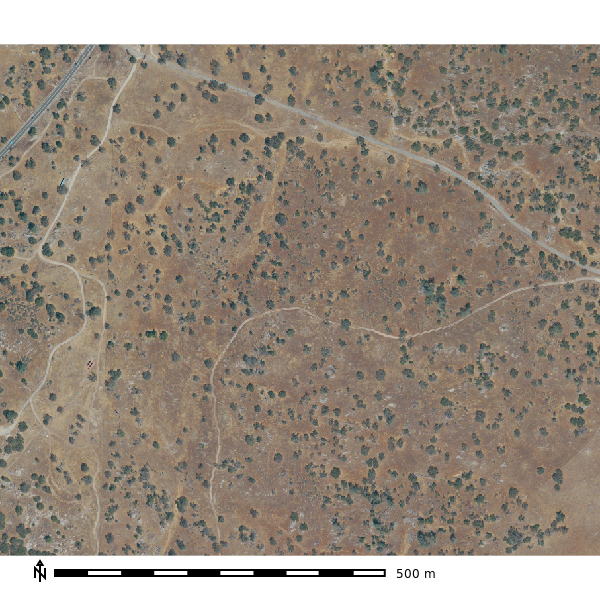
\includegraphics[width=0.45\textwidth,height=\textheight]{../output/SJER/naip.png}
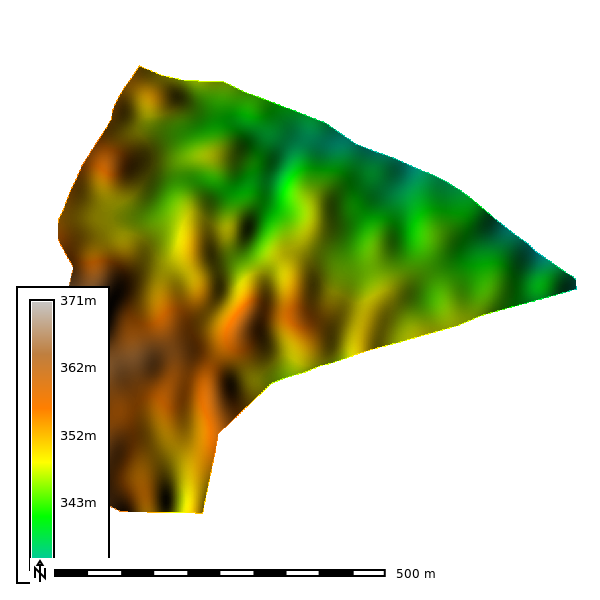
\includegraphics[width=0.45\textwidth,height=\textheight]{../output/SJER/elev.png}
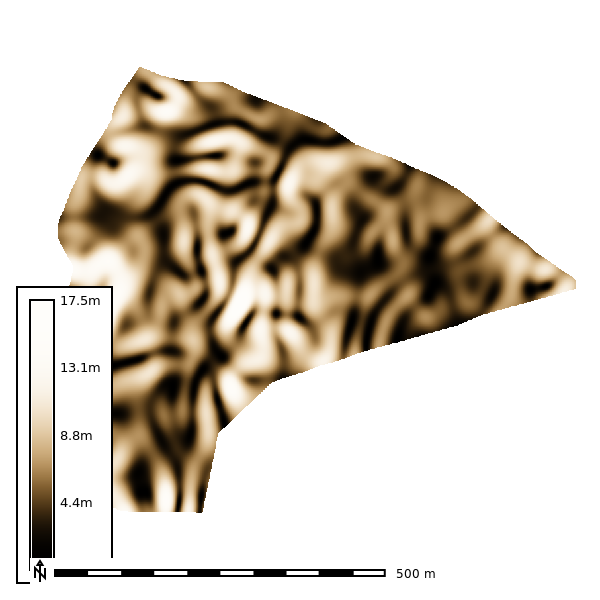
\includegraphics[width=0.45\textwidth,height=\textheight]{../output/SJER/slope.png}
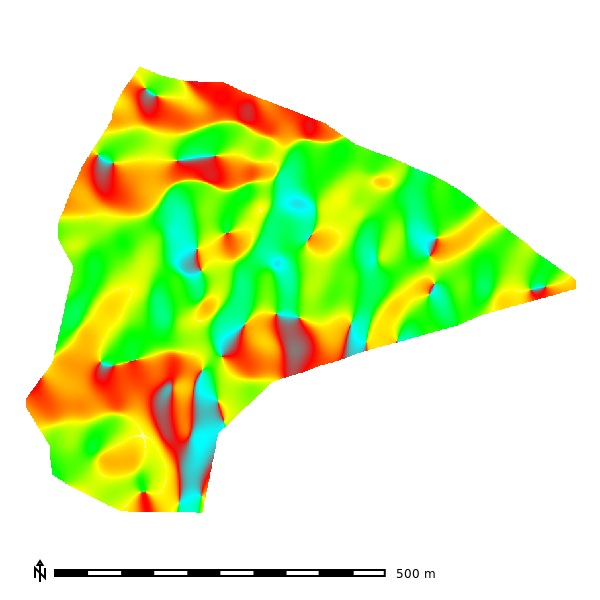
\includegraphics[width=0.45\textwidth,height=\textheight]{../output/SJER/aspect.png}
\end{column}

\begin{column}{0.5\textwidth}
\begin{longtable}[]{@{}ll@{}}
\toprule\noalign{}
Site Details & \\
\midrule\noalign{}
\endhead
EPSG & 26911 \\
Res. & 1 \(m\) \\
Cells & 295,126 \\
Area & 0.3 \(km^2\) \\
ARS & 0.14 \\
\bottomrule\noalign{}
\end{longtable}

\begin{longtable}[]{@{}ll@{}}
\toprule\noalign{}
Elevation & \\
\midrule\noalign{}
\endhead
Min - Max & 333.12 - 371.12 \(m\) \\
Range & 38.0 \(m\) \\
Mean & 349.67 \(m\) \\
Std & 7.96 \\
\bottomrule\noalign{}
\end{longtable}
\end{column}
\end{columns}
\end{block}

\begin{block}{Study Area - Clay Center}
\phantomsection\label{study-area---clay-center}
\begin{columns}[T]
\begin{column}{0.5\textwidth}
\includegraphics[width=0.45\textwidth,height=\textheight]{../output/clay-center/naip.png}
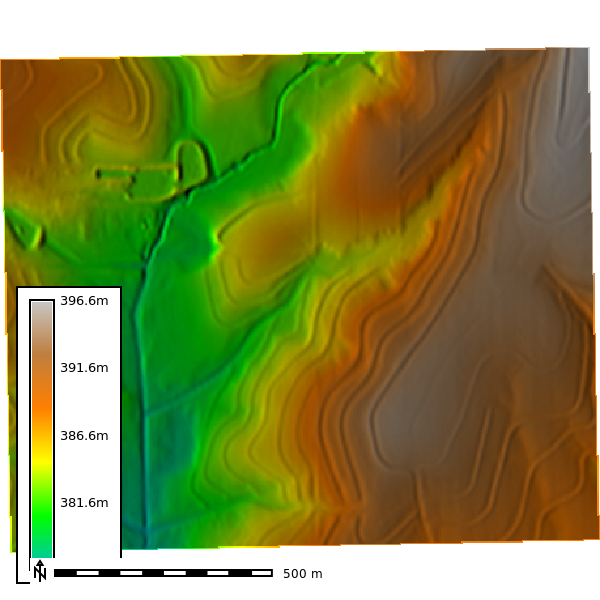
\includegraphics[width=0.45\textwidth,height=\textheight]{../output/clay-center/elev.png}
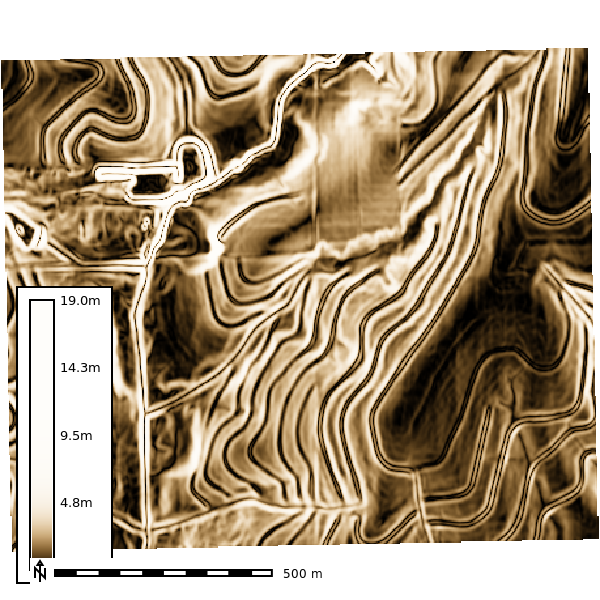
\includegraphics[width=0.45\textwidth,height=\textheight]{../output/clay-center/slope.png}
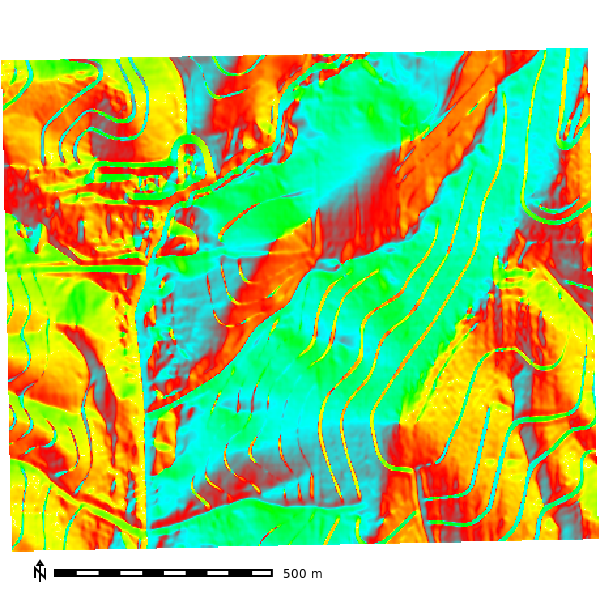
\includegraphics[width=0.45\textwidth,height=\textheight]{../output/clay-center/aspect.png}
\end{column}

\begin{column}{0.5\textwidth}
\begin{longtable}[]{@{}ll@{}}
\toprule\noalign{}
Site Details & \\
\midrule\noalign{}
\endhead
EPSG & 32614 \\
Res. & 3 \(m\) \\
Cells & 170,244 \\
Area & 1.53 \(km^2\) \\
ARS & 0.13 \\
\bottomrule\noalign{}
\end{longtable}

\begin{longtable}[]{@{}ll@{}}
\toprule\noalign{}
Elevation & \\
\midrule\noalign{}
\endhead
Min - Max & 376.69 - 396.57 \(m\) \\
Range & 19.9 \(m\) \\
Mean & 386.71 \(m\) \\
Stddev & 5.03 \\
\bottomrule\noalign{}
\end{longtable}
\end{column}
\end{columns}
\end{block}

\begin{block}{Study Area - Coweeta}
\phantomsection\label{study-area---coweeta}
\begin{columns}[T]
\begin{column}{0.5\textwidth}
\includegraphics[width=0.45\textwidth,height=\textheight]{../output/coweeta//naip.png}
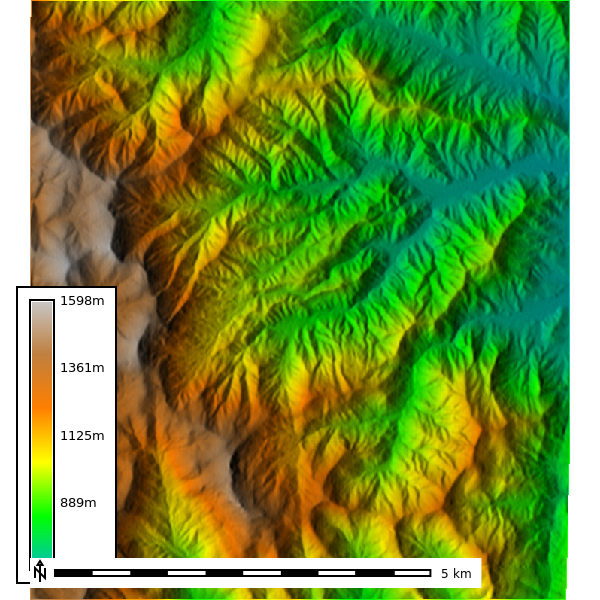
\includegraphics[width=0.45\textwidth,height=\textheight]{../output/coweeta/elev.png}
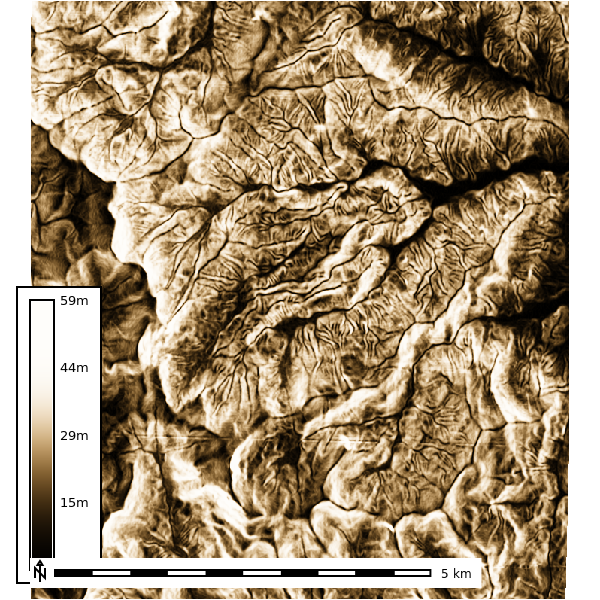
\includegraphics[width=0.45\textwidth,height=\textheight]{../output/coweeta/slope.png}
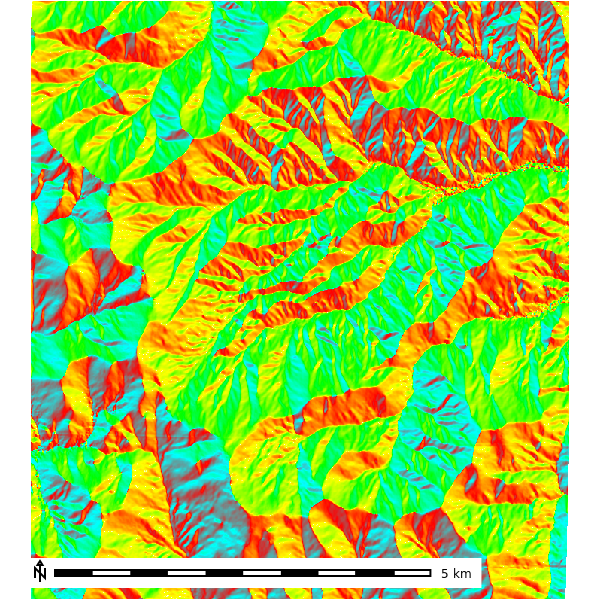
\includegraphics[width=0.45\textwidth,height=\textheight]{../output/coweeta/aspect.png}
\end{column}

\begin{column}{0.5\textwidth}
\begin{longtable}[]{@{}ll@{}}
\toprule\noalign{}
Site Details & \\
\midrule\noalign{}
\endhead
EPSG & 26917 \\
Res. & 10 \(m\) \\
Cells & 572,246 \\
Area & 57.17 \(km^2\) \\
ARS & 5.5 \\
\bottomrule\noalign{}
\end{longtable}

\begin{longtable}[]{@{}ll@{}}
\toprule\noalign{}
Elevation & \\
\midrule\noalign{}
\endhead
Min - Max & 652.8 - 1597.6 \(m\) \\
Range & 944.8 \(m\) \\
Mean & 1043.83 \(m\) \\
Stddev & 230.3 \\
\bottomrule\noalign{}
\end{longtable}
\end{column}
\end{columns}
\end{block}

\begin{block}{Study Area - SFREC}
\phantomsection\label{study-area---sfrec}
\begin{columns}[T]
\begin{column}{0.5\textwidth}
\includegraphics[width=0.45\textwidth,height=\textheight]{../output/SFREC//naip.png}
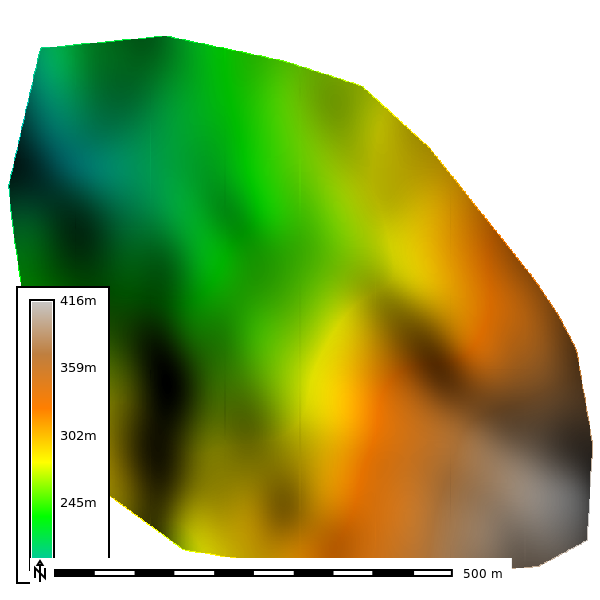
\includegraphics[width=0.45\textwidth,height=\textheight]{../output/SFREC/elev.png}
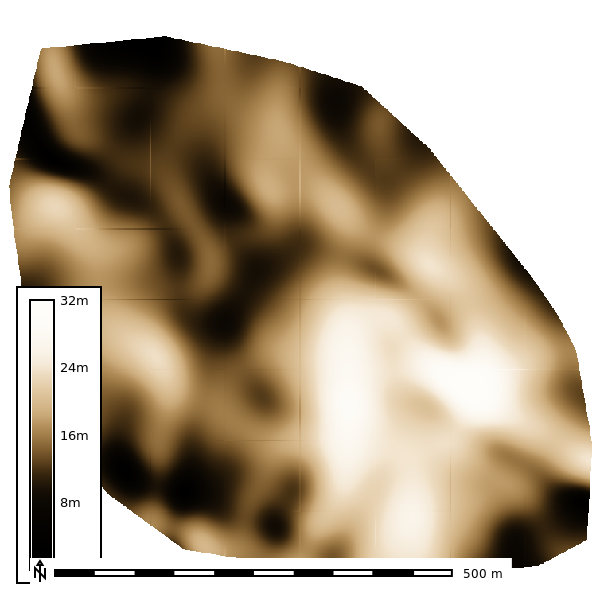
\includegraphics[width=0.45\textwidth,height=\textheight]{../output/SFREC/slope.png}
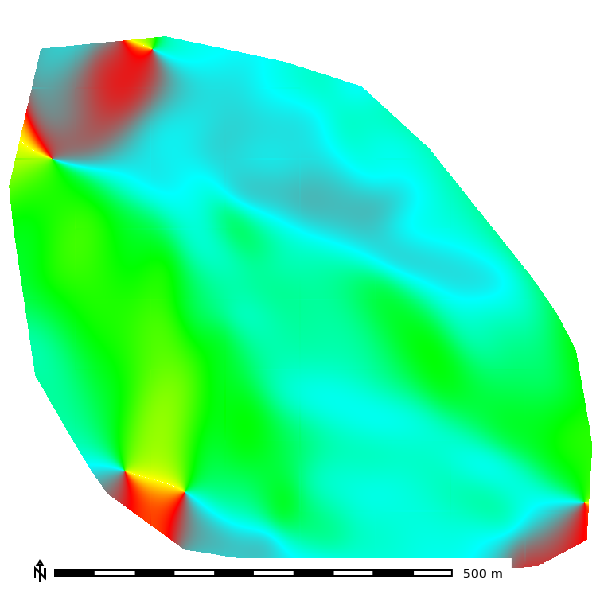
\includegraphics[width=0.45\textwidth,height=\textheight]{../output/SFREC/aspect.png}
\end{column}

\begin{column}{0.5\textwidth}
\begin{longtable}[]{@{}ll@{}}
\toprule\noalign{}
Site Details & \\
\midrule\noalign{}
\endhead
EPSG & 26910 \\
Res. & 1 \(m\) \\
Cells & 380,014 \\
Area & 0.38 \(km^2\) \\
ARS & 0.37 \\
\bottomrule\noalign{}
\end{longtable}

\begin{longtable}[]{@{}ll@{}}
\toprule\noalign{}
Elevation & \\
\midrule\noalign{}
\endhead
Min - Max & 188.61 - 415.64 \(m\) \\
Range & 227.03 \(m\) \\
Mean & 282.1 \(m\) \\
Stddev & 56.1 \\
\bottomrule\noalign{}
\end{longtable}
\end{column}
\end{columns}
\end{block}

\begin{block}{Study Area - tx069-playas}
\phantomsection\label{study-area---tx069-playas}
\begin{columns}[T]
\begin{column}{0.5\textwidth}
\includegraphics[width=0.45\textwidth,height=\textheight]{../output/tx069-playas//naip.png}
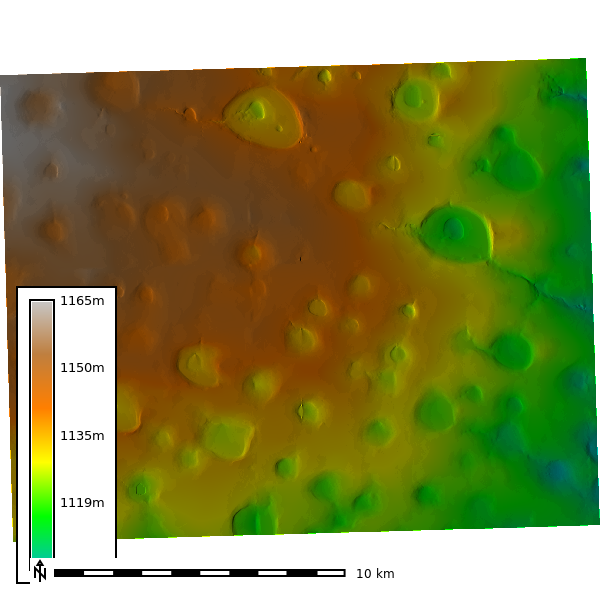
\includegraphics[width=0.45\textwidth,height=\textheight]{../output/tx069-playas/elev.png}
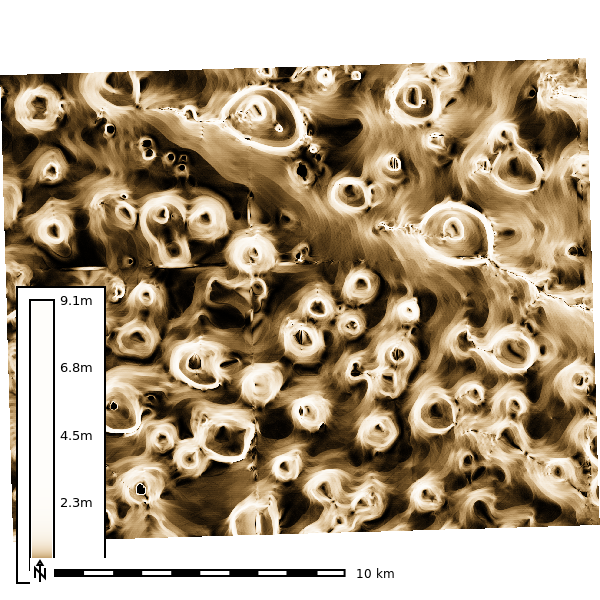
\includegraphics[width=0.45\textwidth,height=\textheight]{../output/tx069-playas/slope.png}
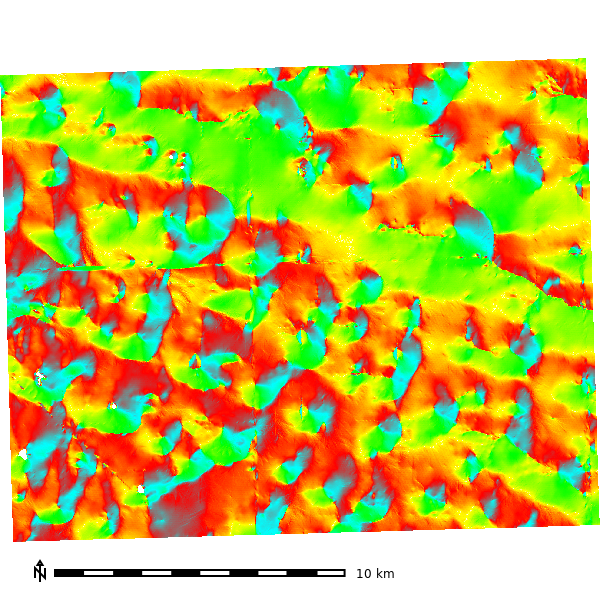
\includegraphics[width=0.45\textwidth,height=\textheight]{../output/tx069-playas/aspect.png}
\end{column}

\begin{column}{0.5\textwidth}
\begin{longtable}[]{@{}ll@{}}
\toprule\noalign{}
Site Details & \\
\midrule\noalign{}
\endhead
EPSG & 32613 \\
Res. & 8 \(m\) \\
Cells & 5,378,306 \\
Area & 324.74 \(km^2\) \\
ARS & 0.07 \\
\bottomrule\noalign{}
\end{longtable}

\begin{longtable}[]{@{}ll@{}}
\toprule\noalign{}
Elevation & \\
\midrule\noalign{}
\endhead
Min - Max & 1104.0 - 1165.3 \(m\) \\
Range & 61.3 \(m\) \\
Mean & 1134.9 \(m\) \\
Stddev & 13.13 \\
\bottomrule\noalign{}
\end{longtable}
\end{column}
\end{columns}
\end{block}

\begin{block}{Study Areas}
\phantomsection\label{study-areas}
\begin{columns}[T]
\begin{column}{0.4\textwidth}
\begin{longtable}[]{@{}ll@{}}
\toprule\noalign{}
Site & ARS \\
\midrule\noalign{}
\endhead
\textbf{tx069-playas} & 0.07 \\
clay-center & 0.13 \\
SJER & 0.14 \\
SFREC & 0.37 \\
\textbf{Coweeta} & 5.5 \\
\bottomrule\noalign{}
\end{longtable}
\end{column}

\begin{column}{0.6\textwidth}
\begin{figure}[H]

{\centering 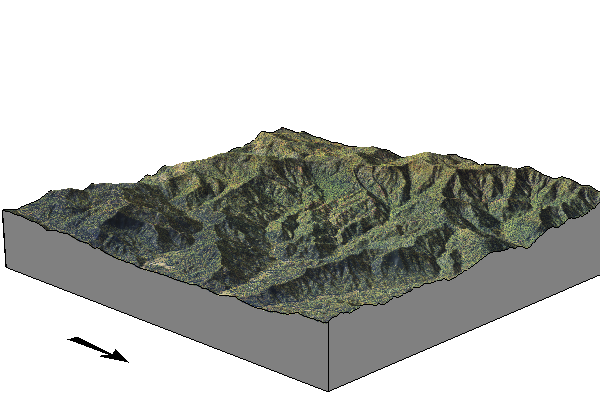
\includegraphics{../output/coweeta/elevation_3dmap.png}

}

\caption{Coweeta}

\end{figure}%
\end{column}
\end{columns}
\end{block}

\begin{block}{Preliminary Results}
\phantomsection\label{preliminary-results}
\textbf{Evaluating}

\begin{itemize}
\tightlist
\item
  SJER
\item
  Clay-Center
\end{itemize}
\end{block}

\begin{block}{Compute Time}
\phantomsection\label{compute-time}
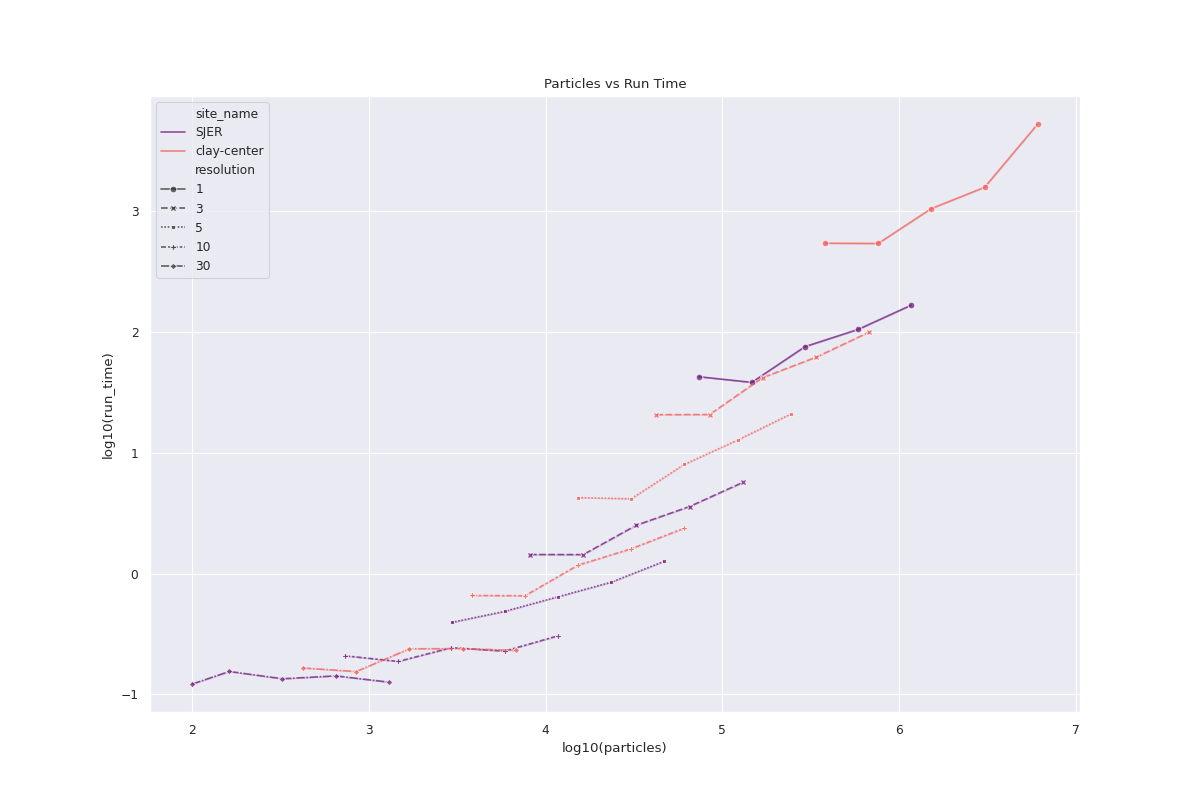
\includegraphics{../output/agu2024_particles_run_time.png}

\begin{quote}
Particles have a greater impact on compute time than resolution.
\end{quote}
\end{block}
\end{frame}

\begin{frame}{Spatial Patterns of Overland Flow}
\phantomsection\label{spatial-patterns-of-overland-flow}
\begin{block}{SJER - Mean Depth}
\phantomsection\label{sjer---mean-depth}
1m Resolution, Particle Density: 4x

\includegraphics{../output/SJER/sensitivity_1/SJER_depth_1_4_s_average.webp}
\end{block}

\begin{block}{SJER}
\phantomsection\label{sjer}
SJER - Mean Depth, 1m Resolution, Particle Density: 4x

\begin{figure}[H]

{\centering 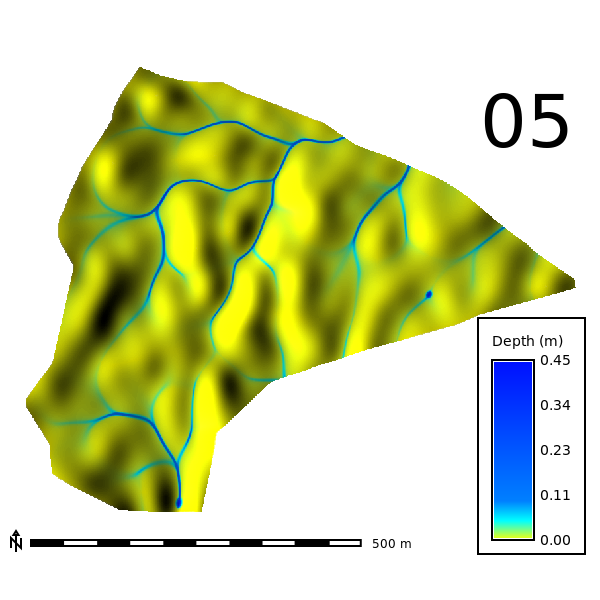
\includegraphics[width=2.08333in,height=\textheight]{../output/SJER/sensitivity_1/SJER_depth_1_4_s_05_average.png}

}

\caption{5 Min}

\end{figure}%

\begin{figure}[H]

{\centering 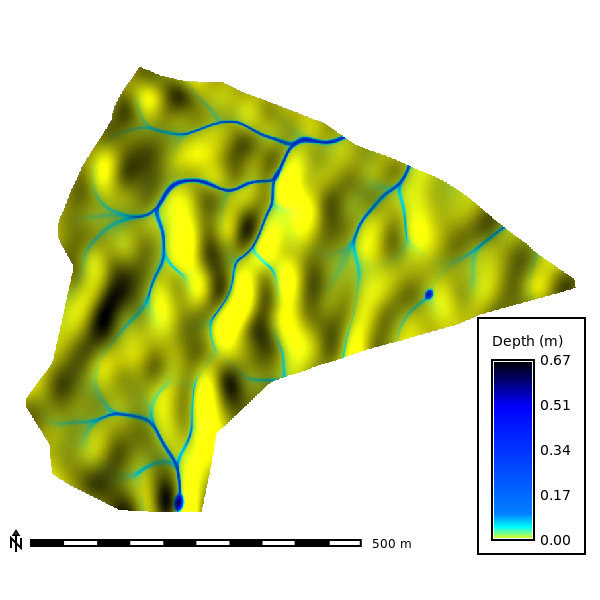
\includegraphics[width=2.08333in,height=\textheight]{../output/SJER/sensitivity_1/SJER_depth_1_4_s_10_average.png}

}

\caption{10 Min}

\end{figure}%

\begin{figure}[H]

{\centering 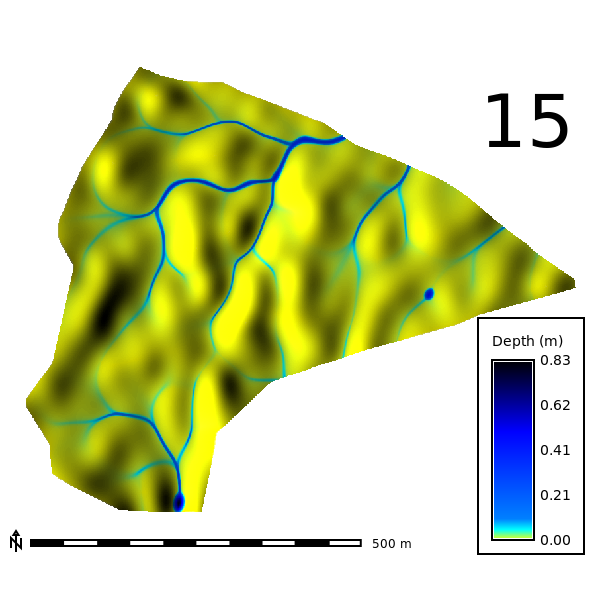
\includegraphics[width=2.08333in,height=\textheight]{../output/SJER/sensitivity_1/SJER_depth_1_4_s_15_average.png}

}

\caption{15 Min}

\end{figure}%

\begin{figure}[H]

{\centering 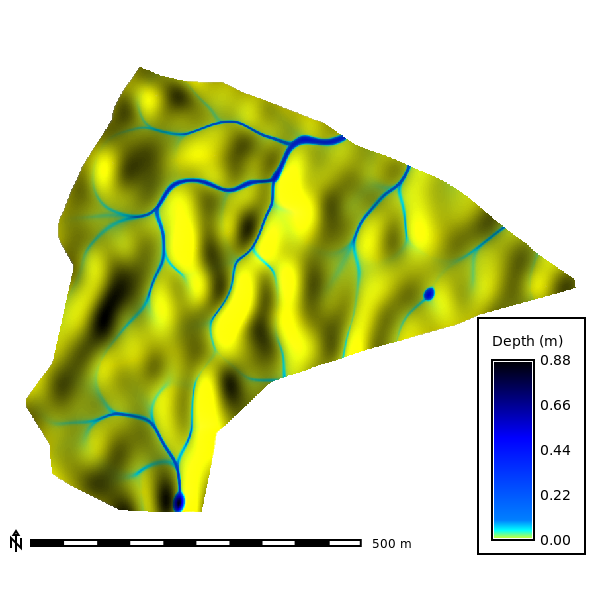
\includegraphics[width=2.08333in,height=\textheight]{../output/SJER/sensitivity_1/SJER_depth_1_4_s_20_average.png}

}

\caption{20 Min}

\end{figure}%

\begin{figure}[H]

{\centering 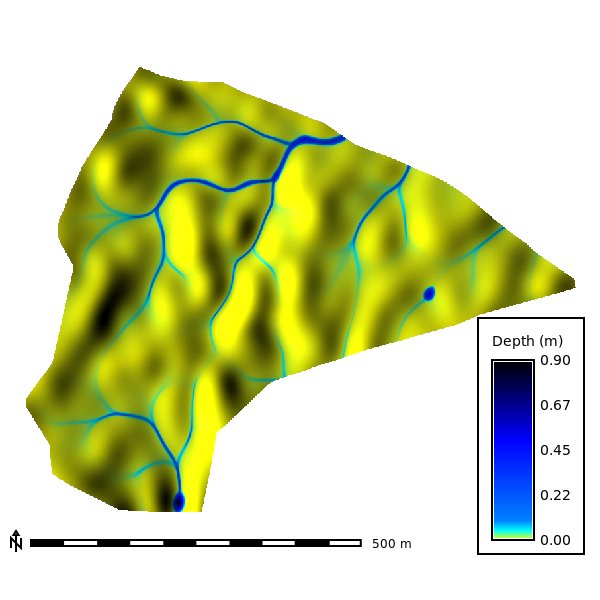
\includegraphics[width=2.08333in,height=\textheight]{../output/SJER/sensitivity_1/SJER_depth_1_4_s_25_average.png}

}

\caption{25 Min}

\end{figure}%

\begin{figure}[H]

{\centering 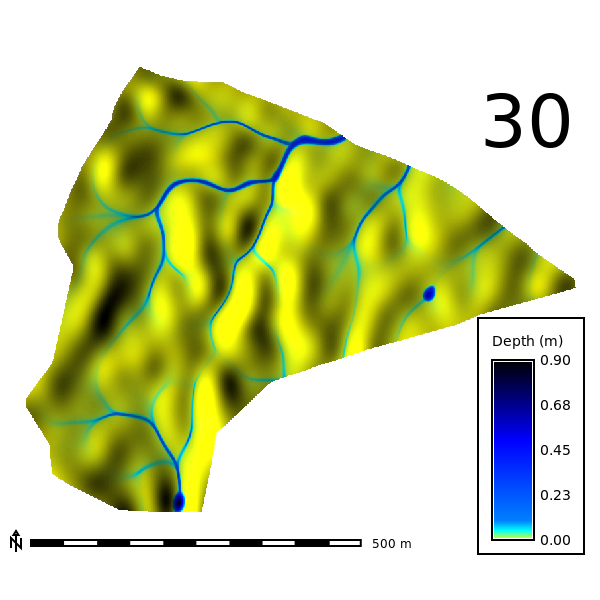
\includegraphics[width=2.08333in,height=\textheight]{../output/SJER/sensitivity_1/SJER_depth_1_4_s_30_average.png}

}

\caption{30 Min}

\end{figure}%
\end{block}

\begin{block}{SJER - Mean Flow Depth}
\phantomsection\label{sjer---mean-flow-depth}
0.25x

\begin{figure}[H]

{\centering \includegraphics{../output/SJER/sensitivity_1/SJER_depth_1_025_s_average.webp}

}

\caption{1m}

\end{figure}%

\begin{figure}[H]

{\centering \includegraphics{../output/SJER/sensitivity_1/SJER_depth_3_025_s_average.webp}

}

\caption{3m}

\end{figure}%

\begin{figure}[H]

{\centering \includegraphics{../output/SJER/sensitivity_1/SJER_depth_5_025_s_average.webp}

}

\caption{5m}

\end{figure}%

\begin{figure}[H]

{\centering \includegraphics{../output/SJER/sensitivity_1/SJER_depth_10_025_s_average.webp}

}

\caption{10m}

\end{figure}%

\begin{figure}[H]

{\centering \includegraphics{../output/SJER/sensitivity_1/SJER_depth_30_025_s_average.webp}

}

\caption{30m}

\end{figure}%

1x

\begin{figure}[H]

{\centering \includegraphics{../output/SJER/sensitivity_1/SJER_depth_1_1_s_average.webp}

}

\caption{1m}

\end{figure}%

\begin{figure}[H]

{\centering \includegraphics{../output/SJER/sensitivity_1/SJER_depth_3_1_s_average.webp}

}

\caption{3m}

\end{figure}%

\begin{figure}[H]

{\centering \includegraphics{../output/SJER/sensitivity_1/SJER_depth_5_1_s_average.webp}

}

\caption{5m}

\end{figure}%

\begin{figure}[H]

{\centering \includegraphics{../output/SJER/sensitivity_1/SJER_depth_10_1_s_average.webp}

}

\caption{10m}

\end{figure}%

\begin{figure}[H]

{\centering \includegraphics{../output/SJER/sensitivity_1/SJER_depth_30_1_s_average.webp}

}

\caption{30m}

\end{figure}%

4.0x

\begin{figure}[H]

{\centering \includegraphics{../output/SJER/sensitivity_1/SJER_depth_1_4_s_average.webp}

}

\caption{1m}

\end{figure}%

\begin{figure}[H]

{\centering \includegraphics{../output/SJER/sensitivity_1/SJER_depth_3_4_s_average.webp}

}

\caption{3m}

\end{figure}%

\begin{figure}[H]

{\centering \includegraphics{../output/SJER/sensitivity_1/SJER_depth_5_4_s_average.webp}

}

\caption{5m}

\end{figure}%

\begin{figure}[H]

{\centering \includegraphics{../output/SJER/sensitivity_1/SJER_depth_10_4_s_average.webp}

}

\caption{10m}

\end{figure}%

\begin{figure}[H]

{\centering \includegraphics{../output/SJER/sensitivity_1/SJER_depth_30_4_s_average.webp}

}

\caption{30m}

\end{figure}%
\end{block}

\begin{block}{Clay Center - Mean Depth}
\phantomsection\label{clay-center---mean-depth}
1m Resolution, Particle Density: 4x

\includegraphics{../output/clay-center/sensitivity_1/clay-center_depth_1_4_s_average.webp}
\end{block}

\begin{block}{Clay Center - Mean Flow Depth}
\phantomsection\label{clay-center---mean-flow-depth}
0.25x

\begin{figure}[H]

{\centering \includegraphics{../output/clay-center/sensitivity_1/clay-center_depth_1_025_s_average.webp}

}

\caption{1m}

\end{figure}%

\begin{figure}[H]

{\centering \includegraphics{../output/clay-center/sensitivity_1/clay-center_depth_3_025_s_average.webp}

}

\caption{3m}

\end{figure}%

\begin{figure}[H]

{\centering \includegraphics{../output/clay-center/sensitivity_1/clay-center_depth_5_025_s_average.webp}

}

\caption{5m}

\end{figure}%

\begin{figure}[H]

{\centering \includegraphics{../output/clay-center/sensitivity_1/clay-center_depth_10_025_s_average.webp}

}

\caption{10m}

\end{figure}%

\begin{figure}[H]

{\centering \includegraphics{../output/clay-center/sensitivity_1/clay-center_depth_30_025_s_average.webp}

}

\caption{30m}

\end{figure}%

1x

\begin{figure}[H]

{\centering \includegraphics{../output/clay-center/sensitivity_1/clay-center_depth_1_1_s_average.webp}

}

\caption{1m}

\end{figure}%

\begin{figure}[H]

{\centering \includegraphics{../output/clay-center/sensitivity_1/clay-center_depth_3_1_s_average.webp}

}

\caption{3m}

\end{figure}%

\begin{figure}[H]

{\centering \includegraphics{../output/clay-center/sensitivity_1/clay-center_depth_5_1_s_average.webp}

}

\caption{5m}

\end{figure}%

\begin{figure}[H]

{\centering \includegraphics{../output/clay-center/sensitivity_1/clay-center_depth_10_1_s_average.webp}

}

\caption{10m}

\end{figure}%

\begin{figure}[H]

{\centering \includegraphics{../output/clay-center/sensitivity_1/clay-center_depth_30_1_s_average.webp}

}

\caption{30m}

\end{figure}%

4.0x

\begin{figure}[H]

{\centering \includegraphics{../output/clay-center/sensitivity_1/clay-center_depth_1_4_s_average.webp}

}

\caption{1m}

\end{figure}%

\begin{figure}[H]

{\centering \includegraphics{../output/clay-center/sensitivity_1/clay-center_depth_3_4_s_average.webp}

}

\caption{3m}

\end{figure}%

\begin{figure}[H]

{\centering \includegraphics{../output/clay-center/sensitivity_1/clay-center_depth_5_4_s_average.webp}

}

\caption{5m}

\end{figure}%

\begin{figure}[H]

{\centering \includegraphics{../output/clay-center/sensitivity_1/clay-center_depth_10_4_s_average.webp}

}

\caption{10m}

\end{figure}%

\begin{figure}[H]

{\centering \includegraphics{../output/clay-center/sensitivity_1/clay-center_depth_30_4_s_average.webp}

}

\caption{30m}

\end{figure}%
\end{block}

\begin{block}{Clay Center - \(3m\) 2x}
\phantomsection\label{clay-center---3m-2x}
\includegraphics{../output/clay-center/sensitivity_1/clay-center_depth_3_2_s_average.webp}
\end{block}

\begin{block}{Clay Center - \(10m\) 2x}
\phantomsection\label{clay-center---10m-2x}
\includegraphics{../output/clay-center/sensitivity_1/clay-center_depth_10_2_s_average.webp}
\end{block}

\begin{block}{Site Depth Comparison}
\phantomsection\label{site-depth-comparison}
\includegraphics[width=0.45\textwidth,height=\textheight]{../output/agu2024_minute_mean_resolution.png}
\includegraphics[width=0.45\textwidth,height=\textheight]{../output/agu2024_minute_max_resolution.png}
\end{block}
\end{frame}

\begin{frame}{What's next?}
\phantomsection\label{whats-next}
\begin{itemize}
\tightlist
\item
  Add additional sites
\item
  Perform statistical analysis
\item
  Include avaliable depth/flow gauge data
\end{itemize}
\end{frame}

\begin{frame}{Questions}
\phantomsection\label{questions}
\end{frame}




\end{document}
